\documentclass{article}
\usepackage{amsmath}
\usepackage{graphicx}
\usepackage{setspace}
\usepackage[affil-it]{authblk}
\usepackage[left=3cm, right=3cm, top=3cm, bottom=3cm]{geometry}
\usepackage{multicol}
\usepackage{listings}
\usepackage[linesnumbered,ruled,vlined]{algorithm2e}
\usepackage{algpseudocode,amsthm}
\usepackage{calrsfs}
\DeclareMathAlphabet{\pazocal}{OMS}{zplm}{m}{n}
% \setlength{\columnsep}{-4cm}
% \usepackage{tikz-qtree}
\usepackage[hidelinks]{hyperref}

\title{CS513: BST Assignment}
\date{}
\author{Prateekshya Priyadarshini}
\affil{M.Tech CSE}
\setcounter{tocdepth}{3}
\begin{document}
\tableofcontents
\newpage
\pagenumbering{arabic}
\maketitle

\section{Approaches}
\subsection{Keeping a dummy node for linked list}
For making addition of nodes easier, one dummy node is created while creating the linked list object. When returning the linked list, the dummy node is first removed and then the list is being returned.
\subsection{Using level order traversal for printing the tree}
Since the order of nodes mentioned in the graphviz file is important, we need to do a traversal of the tree starting from the root such that the root should be mentioned at the top. This can be done using either preorder traversal or level order traversal. Here level order traversal is being considered and a separate queue is implemented for that purpose.
\subsection{Three global variables for printing the tree}
\begin{enumerate}
	\item \textbf{fileCount}\newline
	This variable is initialized to 0. It gets incremented everytime a new graphviz file is created. So that we can create different files each time. For example-graph0.gv,graph1.gv,graph2.gv etc.
	\item \textbf{fileType}\newline
	This variable stores 0 for windows OS, 1 for linux OS. More options can be added as per requirement. This variable helps us to decide which type of commands file we have to create. If we are in windows, we need to add all the commands needed to convert graphviz files to png files into a batch file. Similary in linux we have to add all of them to a shell script.
	\item \textbf{color}\newline
	For reference, after splitting the original tree, both the splitted trees are also being printed. To distinguish between these files, all type of trees which are considered to be the original ones are printed in black, the splitted trees are printed in two different colors i.e. blue and green.
\end{enumerate}
\subsection{Extra variables in Tree Node structure}
To make the tree threaded, there are two boolean variables. They store $true$ if the respective pointer is threaded and $false$ if the pointer points to a legit child.\newline
To get the $k^{th}$ largest element in $O(h)$ time; where $h$ is the height of the tree; there are two integer variables. They store the count of the nodes present in the left subtree and right subtree respectively.
\subsection{Deleting the nodes with two children using successor replacement strategy}
When a node with two children is being deleted, it can be replaced with either with its predecessor or with its successor. Here successor replacement strategy is chosen.
\subsection{Creating batch files or shell scripts}
Since the commands to generate a .png file from a .gv file are not straight forward for a beginner, this program generates batch file in windows and shell script in linux which contains all those commands. Every time a new tree is printed, these files get executed and the respective images get generated. For reference, the images won't be deleted or replaced till the program is being executed.
\subsection{Storing the entire execution process}
The entire execution process is stored in \textbf{output.txt}. This file can be referred to check what went wrong, which images refer to which trees etc.

\section{Files, Functions and Their Logic}
\subsection{nodes.h}
This header file contains node structures for linked list, queue and binary search tree.

\subsection{datastructures.h}
This header file contains linked list class, queue class and binary search tree class along with their respective function prototypes.

\subsection{list.h}
This header file contains the below mentioned functions for linked list.
\subsubsection{void addNode(TreeNode * treeNode)}
This function takes a node of type TreeNode and adds it's data to the end of the linked list. Time complexity is constant.
\subsubsection{void trim()}
This function removes the dummy node from the linked list. Time complexity is constant.

\subsection{queue.h}
This header file contains the below mentioned functions for queue.
\subsubsection{void enqueue(TreeNode * node)}
This function takes a node of type TreeNode and adds the entire node to the queue at the rear end. Time complexity is constant.
\subsubsection{TreeNode * dequeue()}
This function removes and returns the front element of the queue. Time complexity is constant.
\subsubsection{bool isEmpty()}
This function checks whether the queue is empty or not. If the size is zero then it returns true otherwise returns false. Time complexity is constant.
\subsubsection{int getSize()}
This functions returns the current size of the queue. Time complexity is constant.

\subsection{tbst.h}
This header file contains the below mentioned functions for threaded binary search tree.
\subsubsection{void insert(int x)}
This function is called from the main function. It only inserts the node if the root is null. Otherwise it calls another insertion function (Refer \nameref{insertRec}) which uses recursion. It also throws exception if the given value is already present in the tree. The time complexity of this function including the recursion is $O(h)$ where $h$ is the height of the tree.
\subsubsection{TreeNode * search(int x)}
This function is used to search a value in the tree. A pointer is moved from root till leaf according to the given value. If the value is found in the path, then the reference is returned otherwise null is returned. The time complexity of this function is $O(h)$ where $h$ is the height of the tree.
\subsubsection{void deleteX(int x)}
This function deletes a given node. First it searches for the given value. If the value is not present then it throws an exception. Otherwise its parent is searched. There are three possible cases.
\begin{enumerate}
	\item \textbf{Deleting a leaf node}\newline
	This part calls another function (Refer \nameref{deleteLeaf}) which deletes the leaf node and returns the deleted node.
	\item \textbf{Deleting a node having single child}\newline
	This part calls another function (Refer \nameref{deleteSC}) which deletes the required node and returns the deleted node.
	\item \textbf{Deleting a node having two children}\newline
	This part finds out the successor of the current node and the parent of the successor node. Since the successor node can never have a left subtree, not even a left child, so it can be deleted using the functions which delete leaf nodes or nodes having single child. The functions also return the node which is being deleted. So using those functions the successor can be detached from the tree. After that, it is being replaced with the node to be deleted. All the thread information and subtree count information are maintained properly.  
\end{enumerate}
The time complexity for this function is roughly $O(h)$ where $h$ is the height of the tree.
\subsubsection{List reverseInOrder()}
This function uses the threads to find out the reverse inorder traversal. It returns a linked list containing all the values in reverse inorder. No extra stack is being used.

\subsubsection{int successor(TreeNode * xNode)}
This function find out the successor value of a given node. If the given node is the largest node in the tree, it throws an exception. If the given node is null, then also it throws an exception. The time complexity of this function is $O(h)$ where $h$ is the height of the tree.
\subsubsection{TreeNode * split(int k)}
This function splits the tree around a given value k such that all the values in one tree are less than or equal to k and the values in the other tree are greater than k. Then it attaches those trees to a dummy node and returns the dummy node.\newline
The logic of splitting is simple. Maintain two pointers which point to a parent and a child at the same time. If the parent and the child are at two opposite sides of k, that means they will belong to different trees. We need to cut the tree form that point and move the pointers downwards. On the next cut, we need to hold the part being cut using the null pointer of the previous cut. Let's understand this with an example at \textbf{Figure ~\ref{fig:ex1}}.
\begin{figure}
\includegraphics[scale=0.5]{example.png}
\caption{Example tree : red values indicate leaf nodes}
\label{fig:ex1}
\end{figure}
Suppose we are splitting this tree in \textbf{Figure ~\ref{fig:ex1}} around $k=13$. First pointer will point to root i.e. $9$. Now we shall compare $k$ and root. Since k is greater than root, second pointer will point to the right child of root i.e. $15$. We can clearly see that $9$ and $15$ belong to different trees. So we need to make the right child of first pointer $null$. After which the tree will look like \textbf{figure ~\ref{fig:ex2}}. (Of course we have two root pointers one of whom will point to the original root and the other will point to the second node when the first split occurs.)
\begin{figure}
\includegraphics[scale=0.5]{example2.png}
\caption{Example tree : after removing the link from first node}
\label{fig:ex2}
\end{figure}
Here blue and red nodes are first and second nodes respectively. We would have deleted the thread, but since we know $11$ and $9$ will remain in the same tree, there is no need to do that here. Since this was the first split, first root will point to $9$ and the other will point to $15$. The subtree counts are being maintained properly.\newline We shall now move first pointer to second and second to the next level. Since $13$ is less than $15$, second pointer will move to left i.e. $11$. Now $15$ and $11$ also belong to different trees. So we need to make another cut.\newline But the important thing here is, since we are now at a tree which is supposed to contain all values greater than $k$, this means the previous cut was made from a tree which was supposed to contain all the values less than or equal to $k$. Also if we are cutting some part of the current tree where first and second pointers are present, then there is no way that the part which will be cut i.e. the part being pointed by the second pointer will have value greater than $k$. That means, the tree from which the previous cut was made and the part which is being cut now, belong to the same tree. That means here, the tree containing $9$ (this was the node from which the first cut was made) and the part containing $11$ (being cut now), belong to the same tree. Also we have come to the right of $9$ and made the right pointer null. So we can attach $11$ to the right of $9$. \textbf{Figure ~\ref{fig:ex3}} shows the process.
\begin{figure}
\includegraphics[scale=0.5]{example3.png}
\caption{Example tree : moving a part from one tree to other}
\label{fig:ex3}
\end{figure}
We didn't delete the thread of $15$ for the same reason. However, in the program, this condition is being checked and the threads are being removed wherever required. Now we shall move first pointer to $11$. Since $13$ is greater than $11$, we shall move second pointer to right. Now both first and second pointers i.e. $11$ and $12$ belong to the same tree, so we need not do anything and we can directly move forward.\newline
Now first will point to $12$ and second will point to $14$. They both belong to different trees. So we need to $14$. The previous cut was done from $15$. We can again see that, the node from which previous cut was made i.e. $15$ and the node which is being cut now i.e. $14$ belong to the same tree. We had made the left pointer of $15$ $null$. Now it can point to $14$.\newline
This process will continue till first pointer reaches a leaf node. And the resultant trees will look similar to what is shown in \textbf{Figure ~\ref{fig:ex4}}.
\begin{figure}
\includegraphics[scale=0.5]{example4.png}
\caption{Example tree : two different trees splitted around k}
\label{fig:ex4}
\end{figure}
The time complexity is $O(h)$ since we are moving from root to leaf path.
\subsubsection{List inOrder()}
Since we need to print the inorder traversals of the splitted trees, this function is created. It returns a linked list containing all the values of a tree in inorder.
\subsubsection{List allElementsBetween(int k1, int k2)}
This function returns a linked list containing all elements between $k_1$ and $k_2$ in inorder. The logic here is to spot $k_1$ or a value just greater than $k_1$, $k_2$ or a value just smaller than $k_2$. We can store those two nodes in $k_1node$ and $k_2node$ respectively. Then we can traverse from $k_1node$ to $k_2node$ node using the threads which will take roughly $O(h+N)$ where $N$ is the number of nodes from k1 to $k_2$.\newline
So we traverse from root to leaf using a pointer $temp$ and we keep updating $k_1node$ when $temp$ is less than or equal to current value of $k_1node$ node and $temp$ is also greater than or equal to $k_1$. Similarly we put slightly opposite conditions for $k_2node$ to spot $k_2$.
\subsubsection{int kthElement(int k)}
This function finds out the $k^{th}$ largest element from the tree. Since we are storing the subtree counts in each node, if $k$ is greater than the $leftSubtreeCount+rightSubtreeCount+1$ of root, we can straight away throw an exception. Otherwise we shall compare $k$ with the right subtree count. If $k$ is greater than $rightSubtreeCount+1$, we can subtract this count from $k$ and repeat this process on left subtree, else we can move right. When $rightSubtreeCount+1$ and $k$ become equal we return the current node data. This takes $O(h)$ time where $h$ is the height of the tree. 
\subsubsection{void printTree()}
This function does a level order traversal of the tree and generates two files. One is a graphviz(.gv) file and the other file depends on the operating system we are using. For windows it generates a batch file and for linux it generates a shell script.
\subsubsection{void insertIntoTree(TreeNode * root, int x)}
\label{insertRec}
This function is a standard implementation of a recursive insert function along with proper thread and subtree count management. This runs in $O(h)$ time where $h$ is the height of a tree.
\subsubsection{void reduceSubtreeCount(TreeNode * node)}
This function reduces the respective subtree count from root till the parent of a given node in $O(h)$ time where $h$ is the height of a tree.
\subsubsection{bool isLeaf(TreeNode * node)}
This function returns true if the given node is a leaf otherwise returns false.
\subsubsection{TreeNode * deleteLeafNode(TreeNode * node, TreeNode * parent)}
\label{deleteLeaf}
This function deletes a leaf node and updates the threads of its parent. Then it returns the node which got deleted by resetting all the tree parameters.
\subsubsection{TreeNode * deleteNodeWithSingleChild(TreeNode * node, TreeNode * parent)}
\label{deleteSC}
This function replaces the parent's left or right pointer (the same pointer which points to the node to be deleted) with the child of the node to be deleted. The threads are properly managed. Then it returns the node which got deleted by resetting all the tree parameters.
\subsubsection{TreeNode * leftMost(TreeNode * node)}
This function finds the leftmost node of a given node in $O(h)$ where $h$ is the height of the tree.
\subsubsection{TreeNode * rightMost(TreeNode * node)}
This function finds the rightmost node of a given node in $O(h)$ where $h$ is the height of the tree.
\subsubsection{TreeNode * getParent(TreeNode * node)}
This function finds the parent node of a given node in $O(h)$ where $h$ is the height of the tree.
\subsubsection{TreeNode * copyNodes(TreeNode * root, unorderedmap map)}
This is a recursive function called by the copy constructor which creates a replica of the given tree.

\subsection{functions.h}
This file contains some utility functions which are being used multiple times like printing a linked list or printing a long message.

\section{How to create test cases}
\subsection{User prompt}
After executing the program, a prompt will ask the user to enter a number indicating the current operating system. Then a prompt will be printed mentioning the sequence of operations and some small example test cases. It will ask the user to write a file name. So here the user needs to create a .txt file with a sequence of integers and save it in the same directory. Then the same file name should be given in the prompt. A sample prompt is shown in \textbf{Figure ~\ref{fig:ex5}}. If the last instruction is not to quit the execution, after executing the current .txt file the same prompt will reappear for further execution. A new .txt file can be created and the name can be given. For quitting the execution the last instruction in the .txt file should be $10$. Also, "quit" or "exit" or similar keywords can be given instead of file name to quit the execution. Currently added keywords are - quit, exit, stop, return. More can be added at line number - 64 in BinarySearchTreeImpl.cpp\newline
After splitting the original tree, a prompt will appear asking to replace the current tree with any of the splitted trees and the user has to take the proper action.
\begin{figure}
\includegraphics[scale=0.5]{console.png}
\caption{Sample prompt}
\label{fig:ex5}
\end{figure}
\subsection{Example testcase}
1\newline
9\newline
1\newline
5\newline
1\newline
15\newline
1\newline
3\newline
1\newline
7\newline
1\newline
11\newline
1\newline
17\newline
9\newline
6\newline
10\newline
2\newline
15\newline
5\newline
4\newline
7\newline
9\newline
16\newline
10\newline\newline
The above sequence can be written as a test case in an input file, which indicates the following.\newline
1 (Insert the next value)\newline
9\newline
1 (Insert the next value)\newline
5\newline
1 (Insert the next value)\newline
15\newline
1 (Insert the next value)\newline
3\newline
1 (Insert the next value)\newline
7\newline
1 (Insert the next value)\newline
11\newline
1 (Insert the next value)\newline
17\newline
9 (Print the tree)\newline
6 (Split the tree around next value)\newline
10\newline
2 (Search the next value)\newline
15\newline
5 (Find successor of the last searched value)\newline
4 (Get reverse inorder list)\newline
7 (Find the elements between next value and its next value i.e. 9 and 16)\newline
9\newline
16\newline
10 (Quit)
\section{Instructions to execute the code}
\begin{enumerate}
	\item Be careful while executing the program.
	\item If you're using Dev C++, Follow the steps to support $unordered\_map$. Go to tools--compiler option--general tab--tick mark option (add the following commands when calling compiler)--add -std=c++11 there. Then build and execute the project.
	\item In linux or GNU windows compiler, open the terminal or command prompt and type "g++ BinarySearchTreeImpl.cpp" and hit enter.
	\item Then for linux type "./a.out". For windows type "a.exe" or "BinarySearchTreeImpl.exe" (One of them should work). Hit enter.
	\item Now the prompt will be displayed. Enter 0 or 1 for windows or linus respectively.
	\item Write a .txt file according to the given format and enter the file name there. If you give wrong sequence, it can destroy the execution.
	\item If you give an option to split the tree, there will be another prompt to replace your current tree with any of the splitted ones. Give proper option. Wrong choice can lead to destruction of the execution.
	\item The entire execution process can be visualized in output.txt.
	\item After splitting or printing a tree, you can view the images in the same directory. The file names are written in output.txt.
	\item You can give multiple .txt files one after another. For example- in the first run, you can insert a few nodes and find kth largest element. It will print the result and ask you to give another file name. You can now split the tree around the kth largest element and may be discard the higher half and replace the original root with the lower half and then continue execution.
	\item $10$ is used for quit. Do not write 10 unnecessarily inside the .txt file. It is better to keep it at the end.
	\item You can run the batch file or shell script to manually generate the images.
\end{enumerate}

\section{Testing}
The input files, output files, graphviz files, png files, console sequence everything is attached.
Those files can be referred for better understanding.
The sequence is-\newline
\subsection{input1.txt}
\begin{enumerate}
	\item Insert $18, 10, 30, 6, 14, 22, 34, 2, 12, 16, 24, 32, 36, 4, 28,\\ 60, 26, 38, 50, 44, 42, 46, 1, 3, 5, 7, 9, 11, 13, 15, 17, 19, 21, 20, 25$ in that order.
	\item Print the current tree.
	\item Delete $25$.
	\item Print the current tree.
	\item Delete $60$.
	\item Print the current tree.
	\item Delete $18$.
	\item Print the current tree.
	\item Delete $30$.
	\item Print the current tree.
	\item Print reverse inorder.
	\item Search for $46$.
	\item Get its successor.
	\item Search for $50$.
	\item Get its successor.
	\item Find $9^{th}$ largest element.
\end{enumerate}
It prints the $9^{th}$ largest element which is $28$ in this case. Then according to that input2.txt got created.
\subsection{input2.txt}
\begin{enumerate}
	\item Split around $28$.
\end{enumerate}
Then it displays a prompt asking whether to replace the root. Let's replace the original root with the tree having values less than or equal to $28$ i.e. enter $1$.
\subsection{input3.txt}
\begin{enumerate}
	\item Print the current tree.
	\item Find nodes between $8$ to $25$.
	\item Find $15^{th}$ largest number.
\end{enumerate}
It prints the $15^{th}$ largest element which is $10$ in this case. Then according to that input4.txt got created.
\subsection{input4.txt}
\begin{enumerate}
	\item Split around $10$.
	\item Quit.
\end{enumerate}
Entering $0$ in prompt this time not to replace the root.
\subsection{Console sequence}
\begin{center}
\includegraphics[scale=0.5]{console2.png}
\end{center}
\begin{center}
\includegraphics[scale=0.5]{console3.png}
\end{center}
\begin{center}
\includegraphics[scale=0.5]{console4.png}
\end{center}
\begin{center}
\includegraphics[scale=0.5]{console5.png}
\end{center}
\begin{center}
\includegraphics[scale=0.5]{console6.png}
\end{center}

\subsection{Trees sequence}
\subsubsection{Initial tree}
\begin{center}
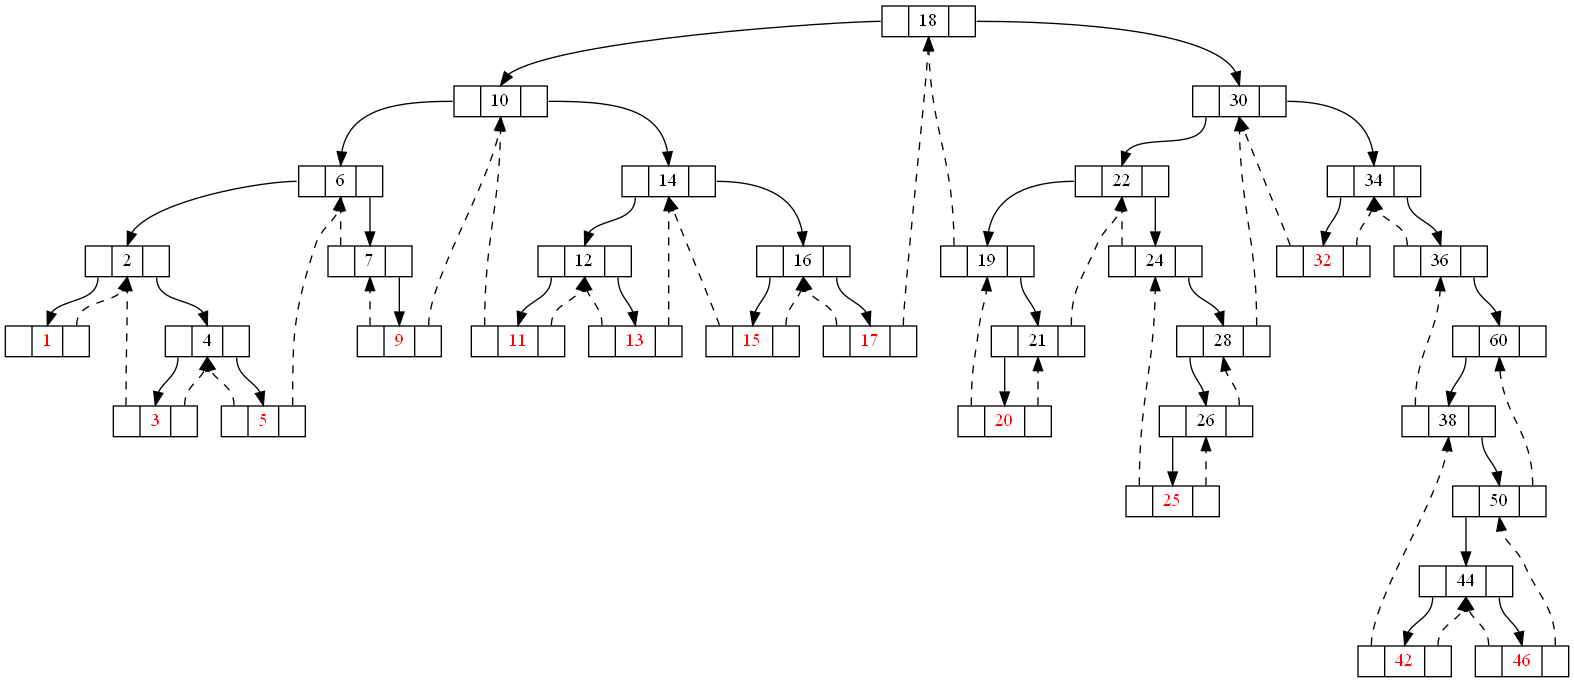
\includegraphics[scale=0.3]{struct0.png}
\end{center}
\subsubsection{After deleting 25}
\begin{center}
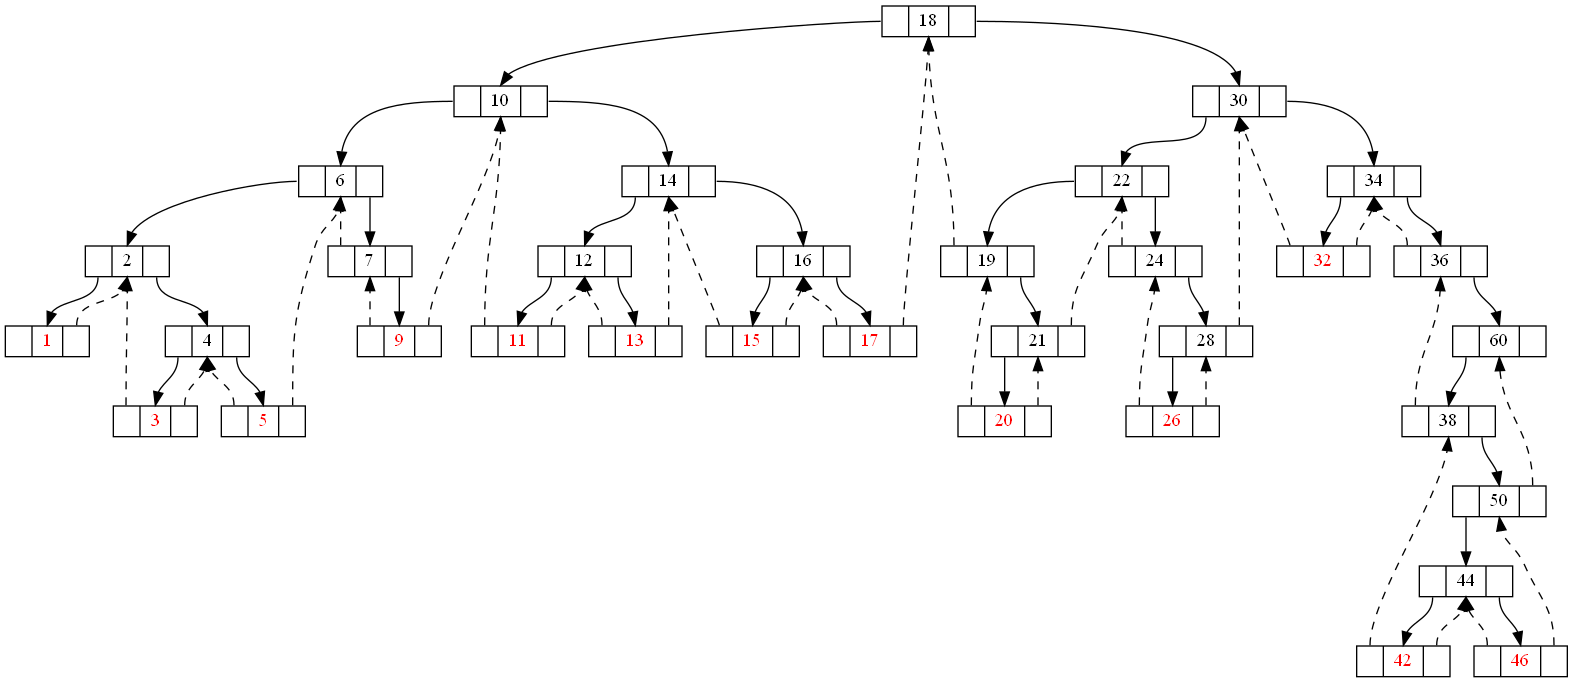
\includegraphics[scale=0.3]{struct1.png}
\end{center}
\subsubsection{After deleting 60}
\begin{center}
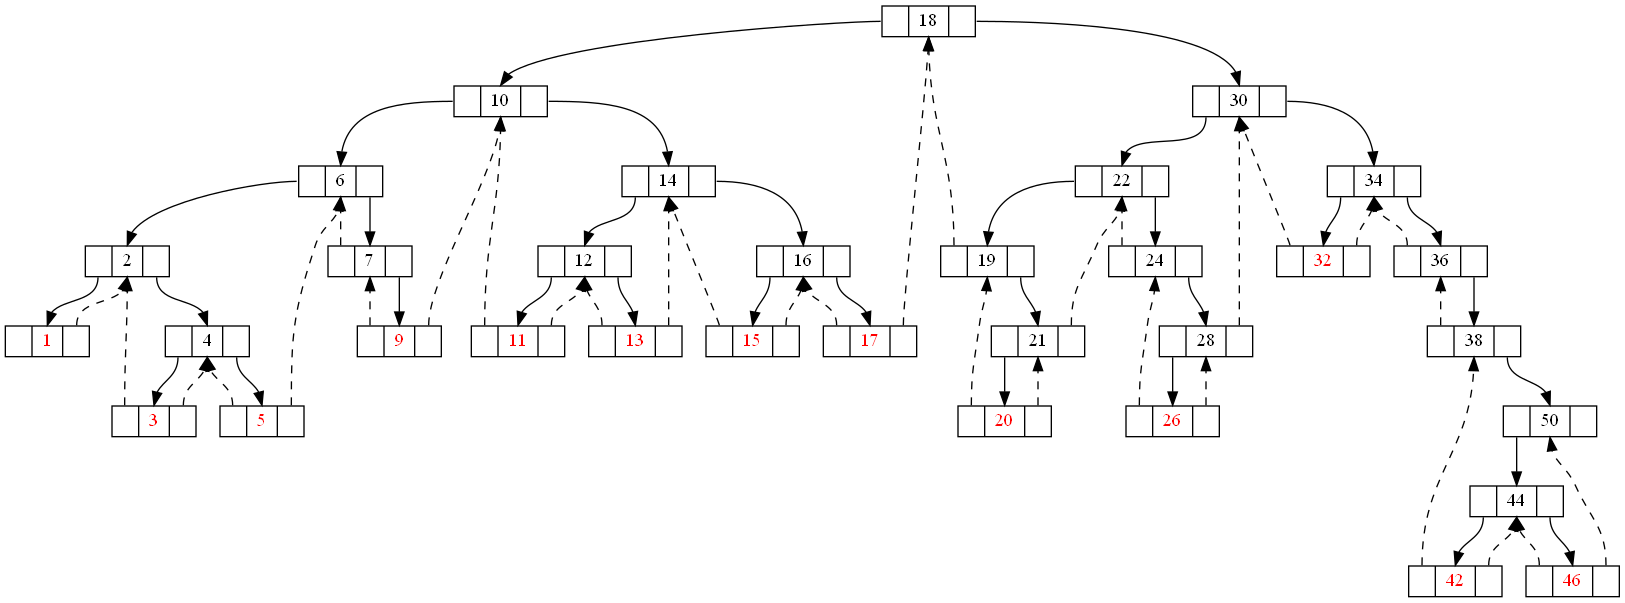
\includegraphics[scale=0.3]{struct2.png}
\end{center}
\subsubsection{After deleting 18}
\begin{center}
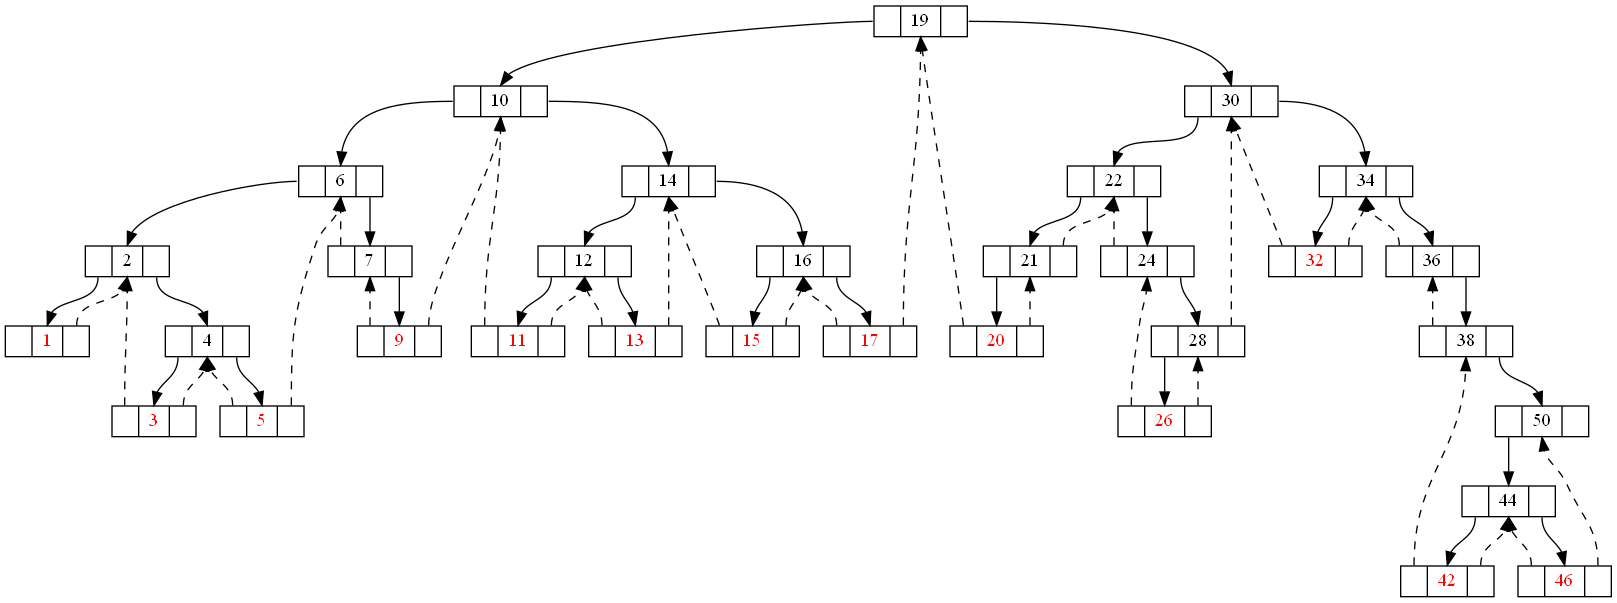
\includegraphics[scale=0.3]{struct3.png}
\end{center}
\subsubsection{After deleting 30}
\begin{center}
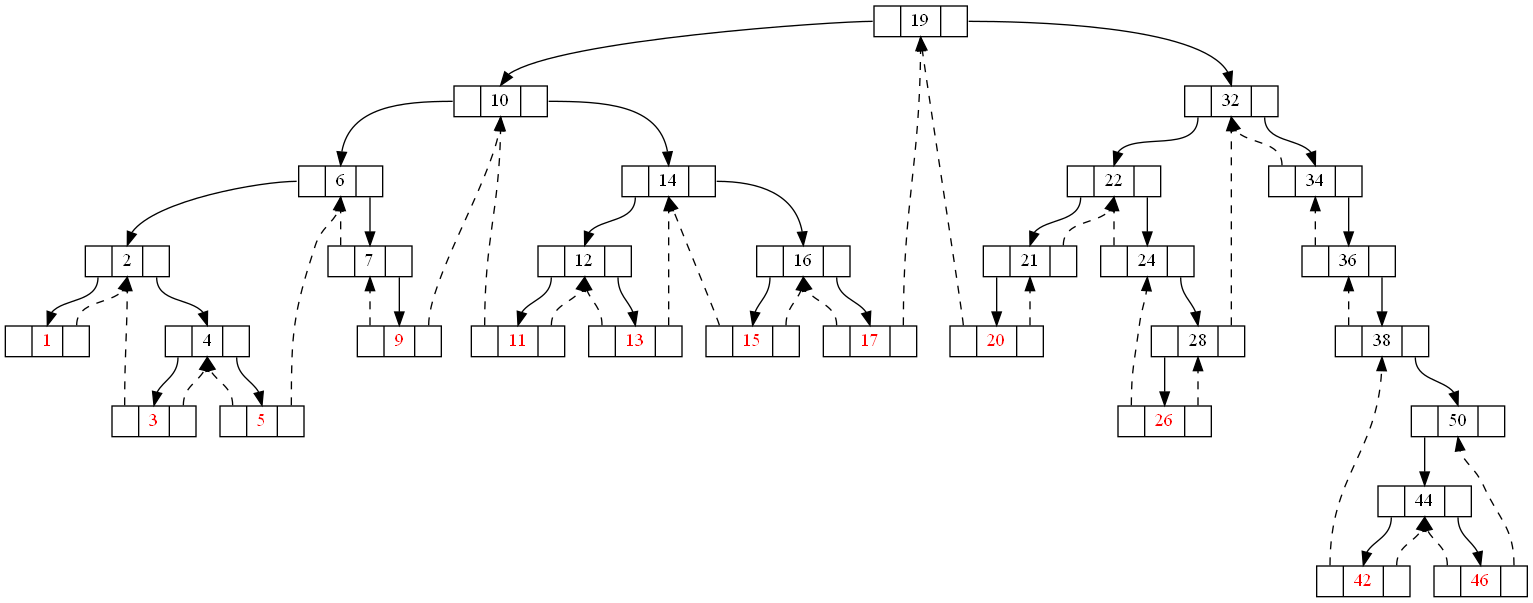
\includegraphics[scale=0.3]{struct4.png}
\end{center}
\subsubsection{After splitting around 28}
\begin{center}
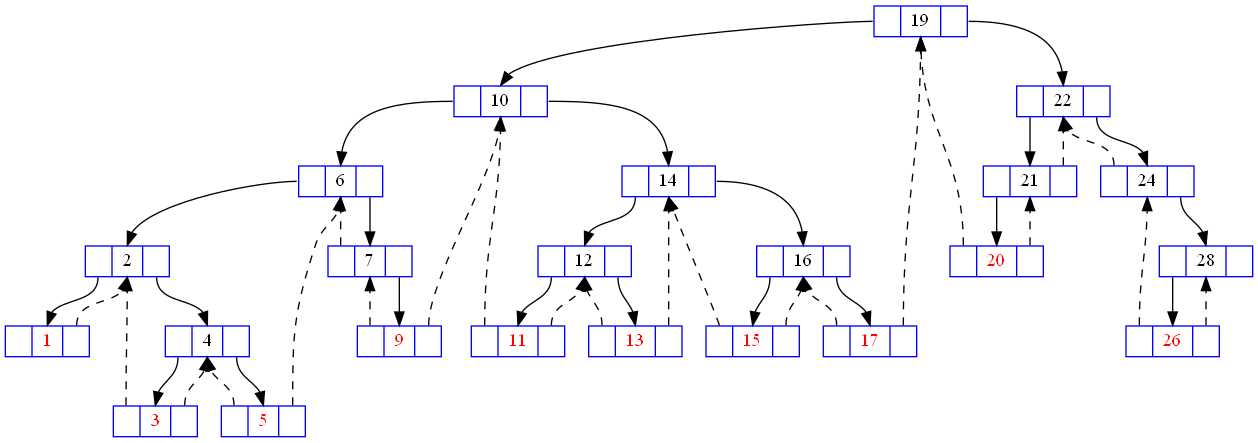
\includegraphics[scale=0.3]{struct5.png}
\end{center}
\begin{center}
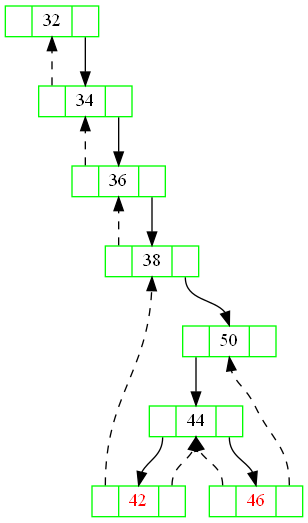
\includegraphics[scale=0.3]{struct6.png}
\end{center}
\subsubsection{After replacing with tree having values $\le 28$}
\begin{center}
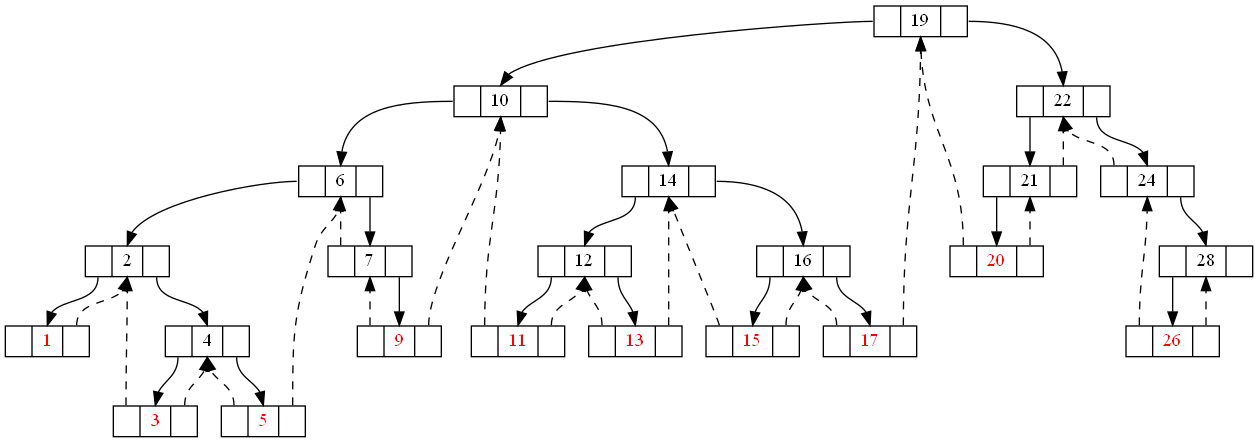
\includegraphics[scale=0.3]{struct7.png}
\end{center}
\subsubsection{After splitting around 10}
\begin{center}
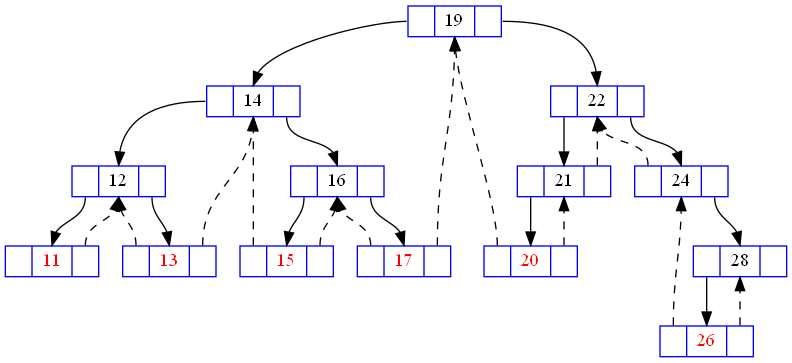
\includegraphics[scale=0.3]{struct8.png}
\end{center}
\begin{center}
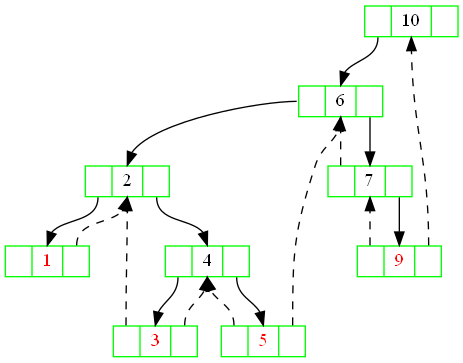
\includegraphics[scale=0.3]{struct9.png}
\end{center}
\end{document}